\documentclass[12pt,onecolumn]{article}

\usepackage{mathptmx}
\usepackage[margin=1in]{geometry}
\usepackage{tabularx}
\usepackage[pdftex]{graphicx}
\usepackage{cite}
\usepackage{amsmath}
\usepackage{microtype}
\usepackage{parskip}
\usepackage{textgreek}
\usepackage{etoolbox}
\usepackage{caption}
\usepackage{subcaption}
\usepackage{float}
\usepackage{multirow}
\usepackage{tocbibind}
\usepackage{enumerate}
\usepackage{listings}
\usepackage{xcolor}

\lstset{frame=tb,
  language=Matlab,
  aboveskip=3mm,
  belowskip=3mm,
  showstringspaces=false,
  columns=flexible,
  basicstyle={\small\ttfamily},
  numbers=none,
  numberstyle=\tiny\color{gray},
  keywordstyle=\color{blue},
  commentstyle=\color{green},
  stringstyle=\color{purple},
  breaklines=true,
  breakatwhitespace=true,
  tabsize=3
}

\usepackage{setspace}
\setstretch{1} 
\usepackage{indentfirst}
\setlength{\parindent}{0pt}
\usepackage{parcolumns}
\setlength{\columnsep}{0.5cm}
\renewcommand*\contentsname{Table of Contents}
\usepackage{fancyhdr}
\pagestyle{fancy}
\fancyhf{}
\lhead{Project 1: Extrema of Functions}
\rhead{\thepage}
\cfoot{}
\fancypagestyle{fancy}{
    \fancyhead{cc} 
    \lhead{}
	\rhead{\thepage}
	\cfoot{}
}



\makeatletter
\renewcommand*\l@section{\@dottedtocline{1}{0em}{1.3em}}
\makeatother

\begin{document}

\begin{titlepage}
\fontsize{20pt}{20pt}\selectfont
\begin{center}
MTE 203 - Advanced Calculus\\
\vspace{4cm}
Project 1\\
\vspace{0.6cm}
Extrema of Functions\\
\end{center}
\vspace{4cm}
Name: Anna Shan\\ \\
Student ID: 20648926\\
\vspace{7cm}
\begin{center}
November 12, 2018
\end{center}

\end{titlepage}

\pagenumbering{roman}
\setcounter{page}{2}

\newpage
\pagenumbering{arabic}
\setcounter{page}{1}

\section{Summary of Analysis}

\subsection*{Part I}

\begin{enumerate}[a.]
\item  A surface plot was used to plot the terrain in 3D. A contour plot with 25 contour lines was generated.
\begin{center}
	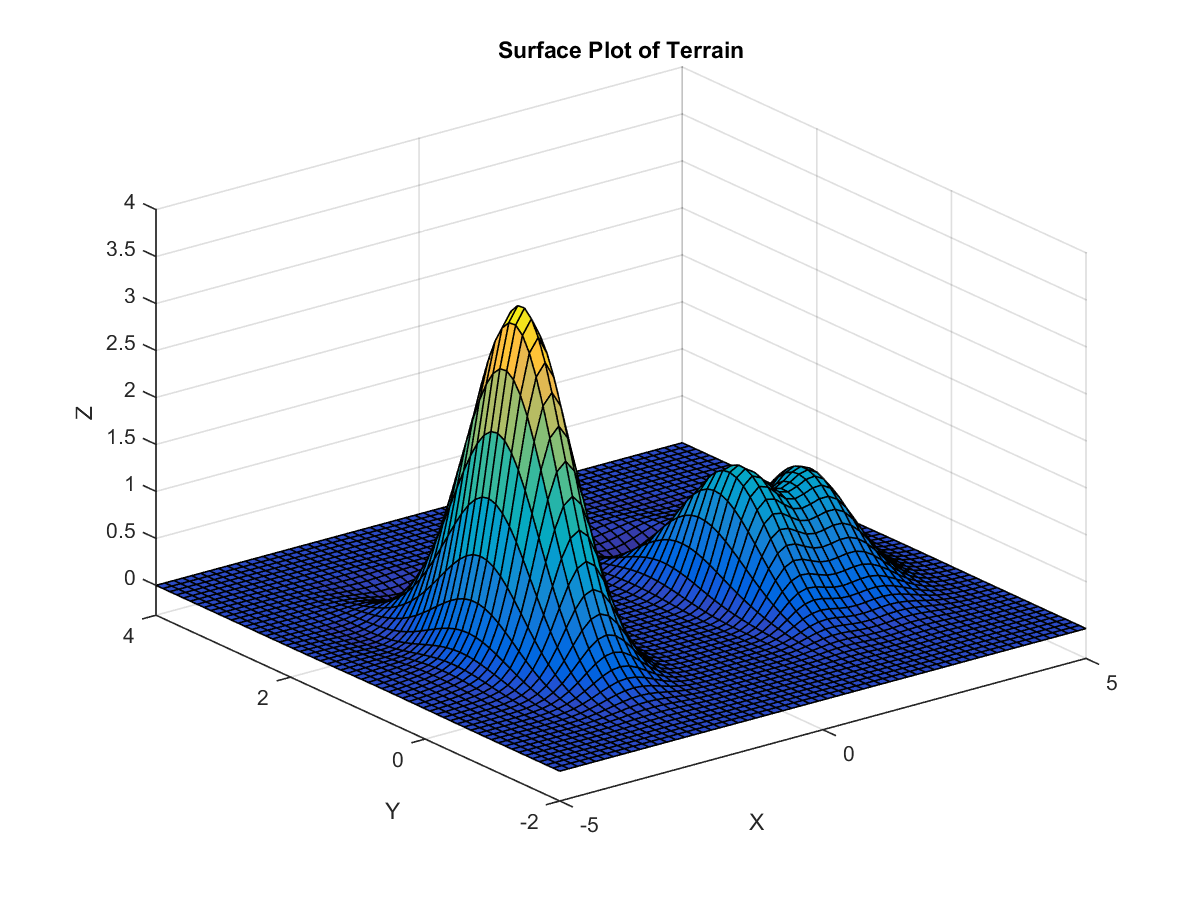
\includegraphics[width=\textwidth]{SurfacePlot}
\end{center}
\begin{center}
	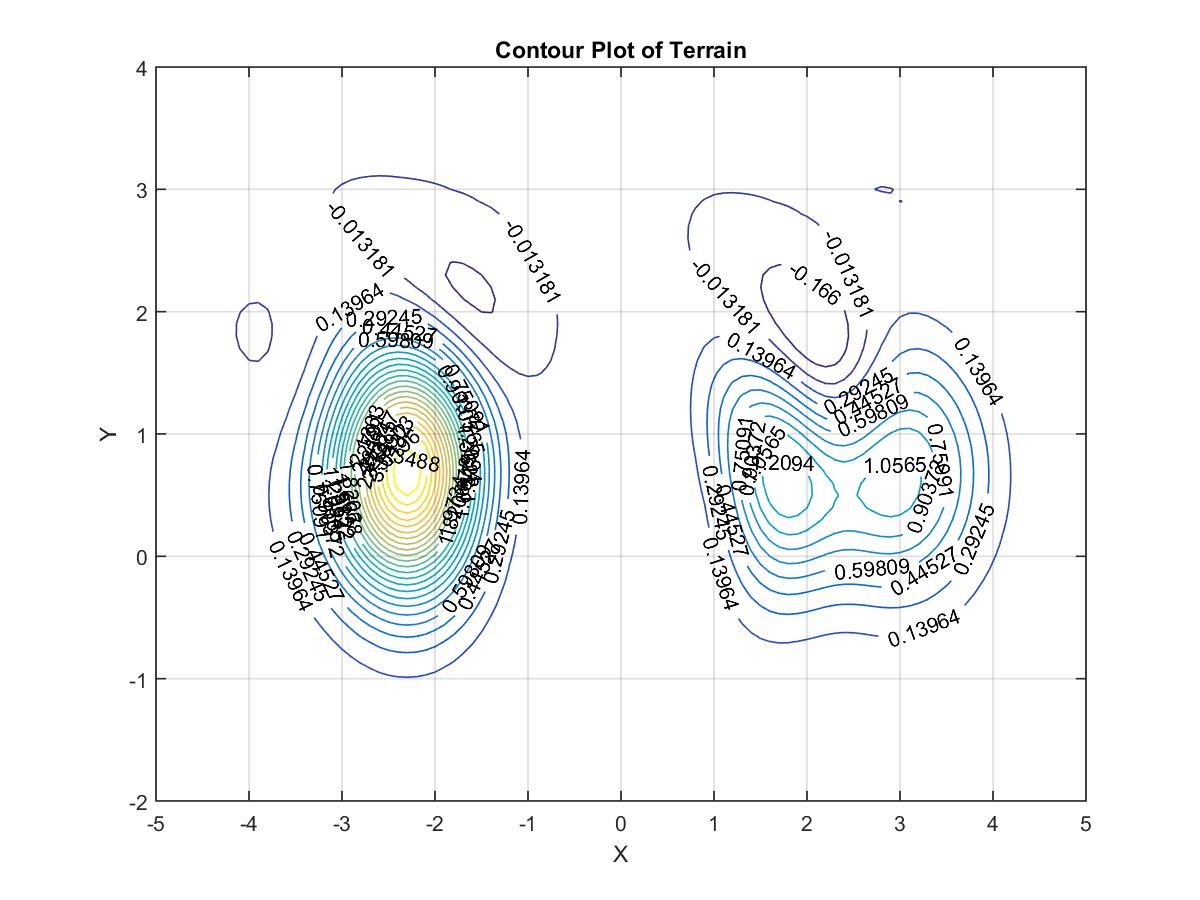
\includegraphics[width=\textwidth]{ContourPlot}
\end{center}

\item The location of the steepest terrain slope can be determined by observing the distance between contour lines. Since the elevation interval is equivalent between lines, the area with the closest contour lines is that with the fastest elevation change. By inspection, the point with the tightest contour lines seems to be located at approximately (-1.8, 0.7).

Mathematically, the steepest slope at any given point is given by the gradient. The coordinates of the steepest terrain slope is thus the location with the maximum gradient length. Using MATLAB, the point was found to be (-1.769, 0.716), which confirms the graphical estimation obtained above.

\item The first partial derivative test was implemented with the following equations:
\begin{align*}
	\frac{\partial f}{\partial x} &= 0\\
	\frac{\partial f}{\partial y} &= 0
\end{align*}
A numerical equation solver (\textit{fsolve} function in MATLAB) was used. A total of 23 critical points were found by iterating over the full range of initial guesses $(x_0, y_0)$ with small increments, where $-5 < x_0 < 5$, $-2 < y_0 < 4$.

The second partial derivative test was implemented using:
\begin{equation*}
	A = \frac{\partial^2f}{\partial x^2};\;\; B = \frac{\partial^2f}{\partial x\partial y};\;\; C = \frac{\partial^2f}{\partial y^2};\;\; D = B^2 - AC
\end{equation*}
The type of critical point $P$ can be determined by the following rules:
\begin{enumerate}[i.]
	\item If $D < 0$, $A < 0$, then $P$ is a relative maximum
	\item If $D < 0$, $A > 0$, then $P$ is a relative minimum
	\item If $D > 0$, then $P$ is a saddle point
	\item If $D = 0$, then $P$ fails the test
\end{enumerate}
The results of the second derivative test are summarised in Table \ref{crit}. Values of $D$ are rounded to 0 when $|D| < 0.01$ to account for rounding and truncation errors.

The maximum and minimum elevations of the terrain are $z = $ 3.655 km, -0.321 km, at points $P = $ (-2.300, 0.687) km, (2.066, 1.893) km, respectively.
\end{enumerate}

\subsection*{Part II}

\begin{enumerate}[a.]
\item Using the provided equation for $T(x,y,f(x,y))$, the temperatures at the highest (-2.300, 0.687) and lowest (2.066, 1.893) elevations are -22.5410$^{\text{o}}$C and 6.3416$^{\text{o}}$C, respectively.

\item
\begin{enumerate}[i.]
\item Using the same approach as $(a)$: $T(2.2,0.5,f(2.2,0.5)) = 4.4959 ^{\text{o}}$C.
\item Isotherms at the specified elevation can be found by setting $z = f(2.2, 0.5)$ and plotting the contour map of $T(x,y,f(2.2,0.5))$:\\
	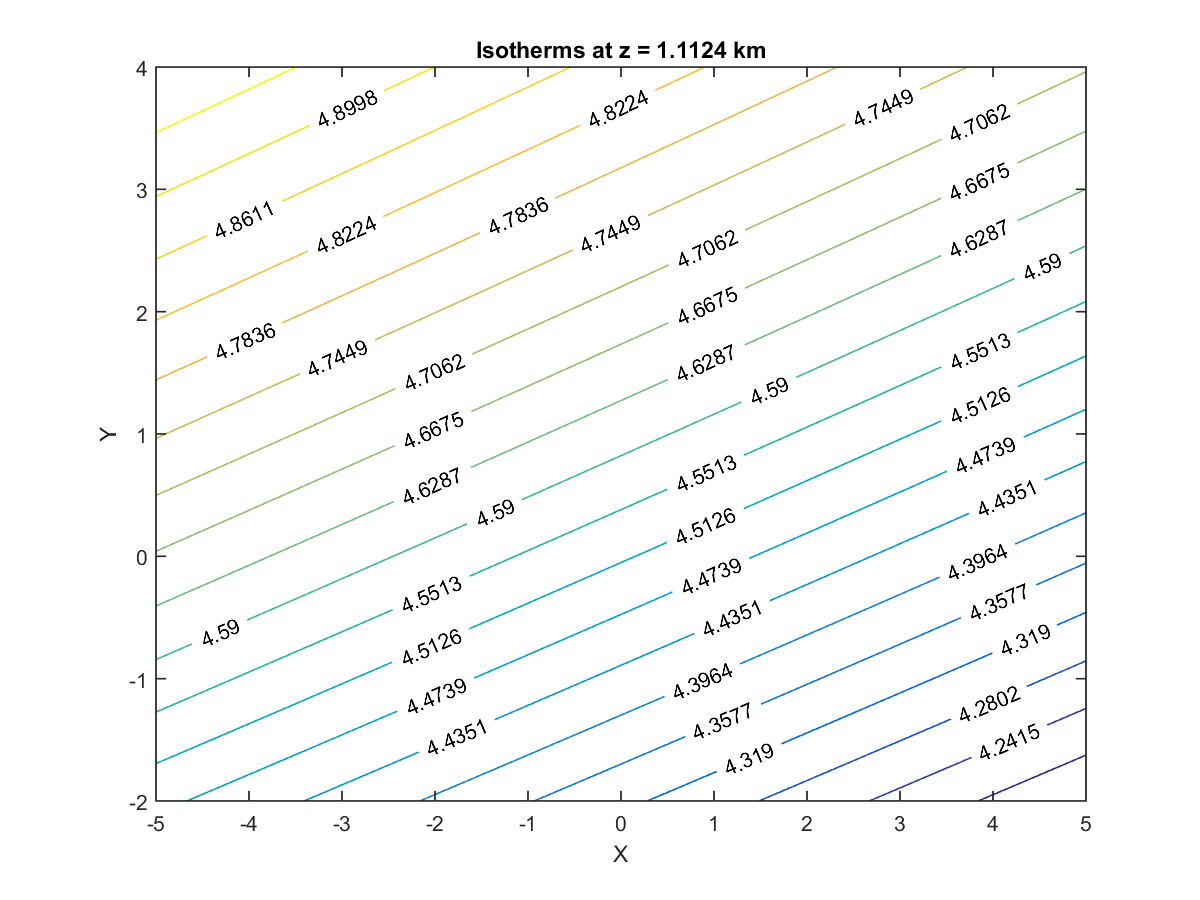
\includegraphics[width=0.9\textwidth]{Isotherms}
\end{enumerate}
\item 
\begin{enumerate}[i.]
\item The rate of change in the north direction can be calculated by the gradient of the function at the specified point in the direction $(0,1)$. The resulting value is 0.0324. A positive value indicates that the hiker would be ascending in this direction.
\item By heading north, the hiker is walking in the $(0, 1, 0.0324)$ direction. The dot product of this direction with the temperature gradient vector at his current location would give the rate of change in temperature along his path. The resulting rate is -0.0560$^{\text{o}}$C/km.
\end{enumerate}
\item 
\begin{enumerate}[i.]
\item The rate of change in the southwest direction can be calculated by the gradient of the function at the specified point in the direction $(-1,-1)$. The resulting value is 0.3904. A positive value indicates that the hiker would be ascending in this direction.
\item By heading southwest, the hiker is walking in the $(-1,-1,0.3904)$ direction. The dot product of this direction with the temperature gradient vector at his current location would give the rate of change in temperature along his path. The resulting rate is -1.2429$^{\text{o}}$C/km.
\end{enumerate}
\newpage
\item Plotting the temperature function as the colour map of the terrain is useful to the hiker because the colour indicates the temperature at a given location.\\
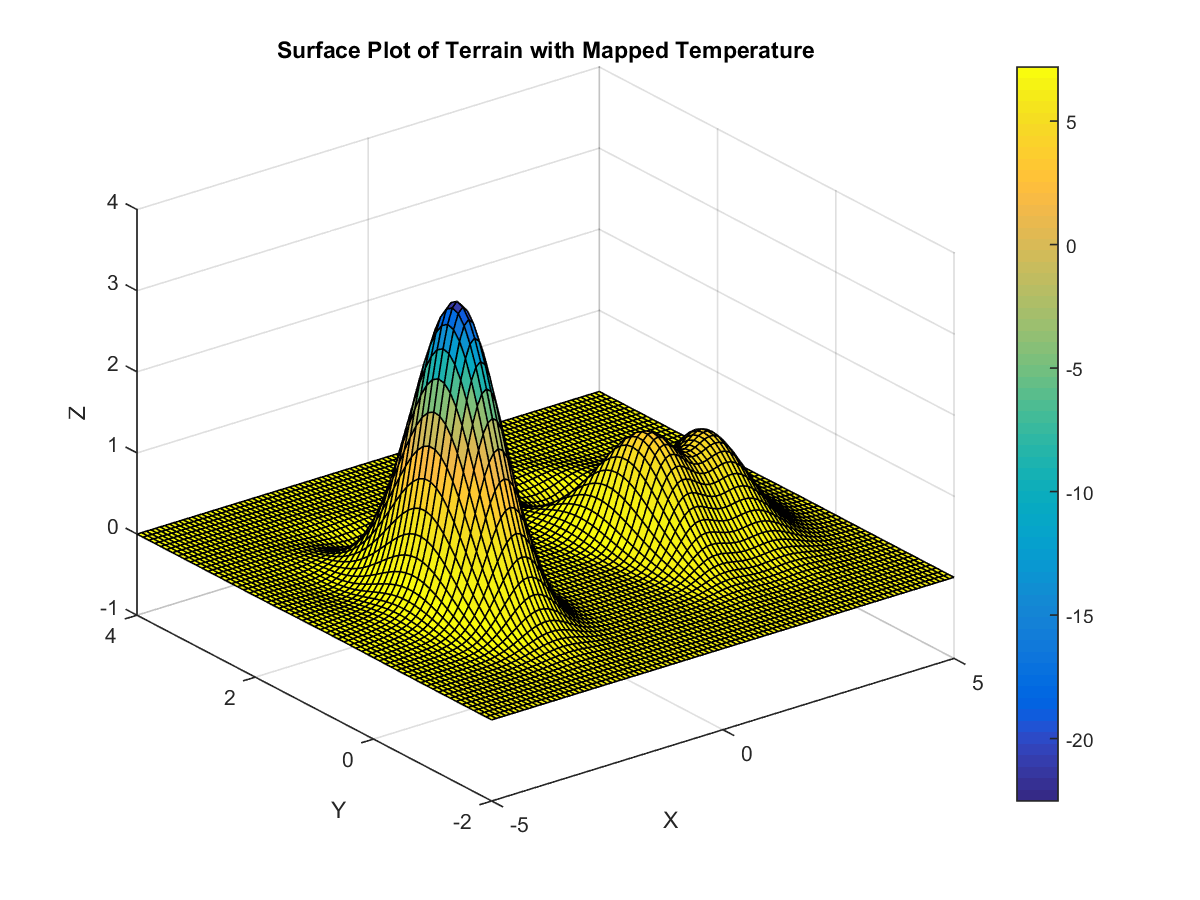
\includegraphics[width=\textwidth]{SurfaceColor}
\item Plotting the temperature function with respect to $x$ and $y$ only is useful to the hiker because the z-axis indicates the temperature at a given $(x,y)$ location with the elevation already taken into account.\\
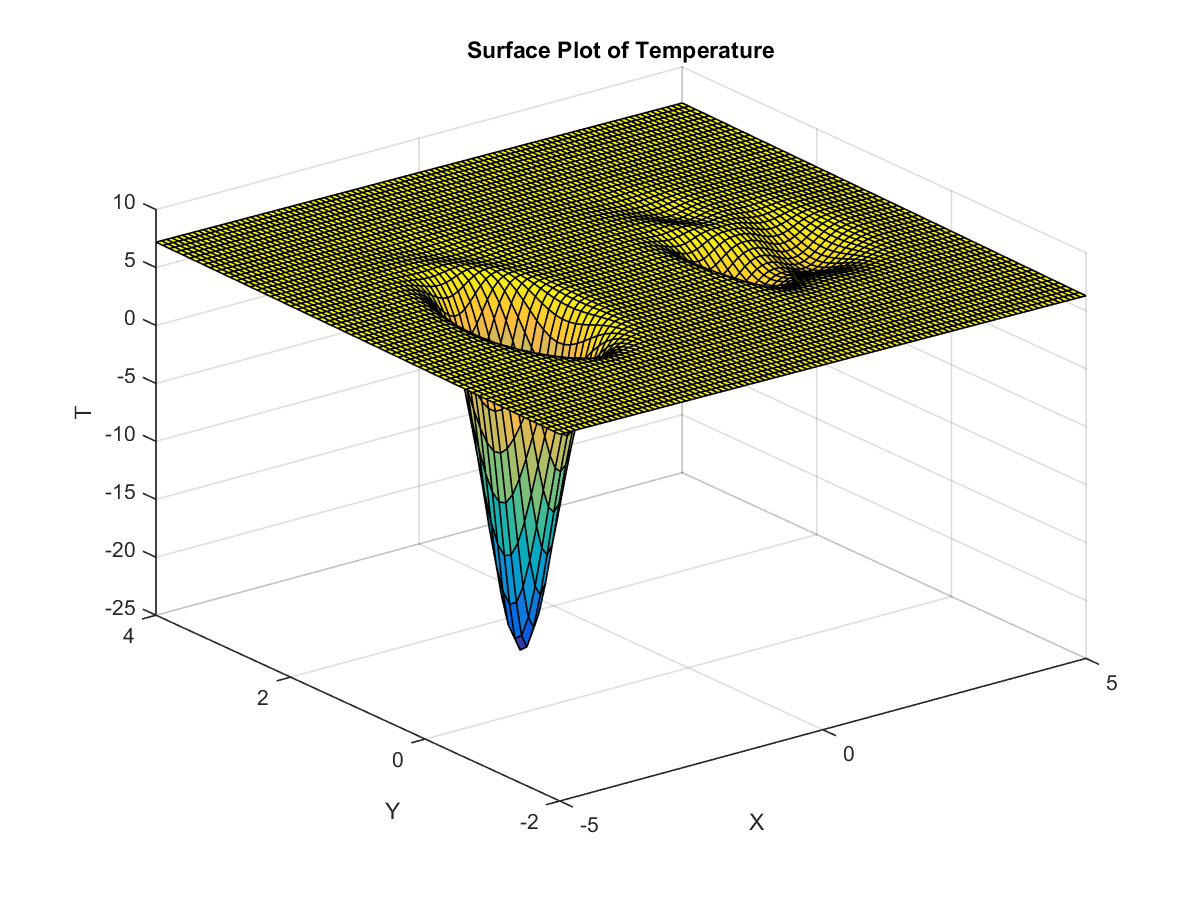
\includegraphics[width=0.9\textwidth]{Temp}
\item Using the Lagrange Multipliers, local extrema of the temperature function can be found with the terrain function used as a constraint:
\begin{align*}
	f(x,y,z)&=10 - 2\, z^2 - \mathrm{e}^{\frac{x}{100} + \frac{{\left(z - 1\right)}^2}{10} + \frac{{\left(\frac{y}{20} - 3\right)}^2}{10} + \frac{1}{5}}\\
	g(x,y,z)&=\mathrm{e}^{ - {\left(y - \frac{4}{5}\right)}^2 - \frac{x^2}{2} - 3}\, \mathrm{log}\!\left(x^4 + 1\right)\, \left(4\, x^4 + 4\, y^2\right)\, \left(2\, \cos\!\left(\frac{3\, y}{4}\right) + \sin\!\left(\frac{y^4}{20} + 2\, x\right)\right)-z = 0
\end{align*}
The local extrema can be found by solving the equations:
\begin{align*}
	\nabla f &= \lambda \nabla g\\
	g(x,y,z) &= 0
\end{align*}
According to the figure in \textit{(e)}, the lowest temperature seems to reside around the highest elevation point. Therefore, the \textit{fsolve} function in MATLAB is used with an initial guess that is somewhere close to the highest elevation point, $(x,y,z)=(-2.3, 0.6, 3.7)$. The exact location was found to be $(x,y,z)=(-2.2995, 0.6863, 3.6551)$ with a temperature of -22.5410$^{\text{o}}$C
\end{enumerate}

\subsection{Problems}

No problems were encountered during the analysis of the project. 

\newpage
\section{Summary of Results}
\begin{table}[H]
\caption {List of Critical Points of the Terrain} \label{crit} 
\begin{tabular}{|c|c|c|c|c|c|c|c|}
\hline
Point \# & $(x, y)$       & $f(x,y)$ & $A$     & $B$    & $C$    & $D = B^2 - AC$ & Type of Point \\ \hline \hline
1        & -3.931, -1.61  & 0        & 0.002   & 0.001  & 0.002  & -3.00E-06      & fail          \\ \hline
2        & -3.902, 1.807  & -0.0190  & 0.314   & -0.011 & 0.203  & -0.063621      & min           \\ \hline
3        & -4.134, 2.869  & 0        & -0.003  & -0.010 & -0.017 & 4.90E-05       & fail          \\ \hline
4        & -2.300, 0.687  & 3.655    & -13.124 & 0.040  & -8.697 & -114.137828    & max           \\ \hline
5        & -1.606, 2.193  & -0.190   & 1.153   & 0.992  & 1.959  & -1.274663      & min           \\ \hline
6        & -1.562, 3.131  & -0.003   & -0.025  & -0.090 & -0.228 & 0.0024         & fail          \\ \hline
7        & -1.251, -1.773 & 0        & 0.005   & -0.005 & 0.008  & -1.50E-05      & fail          \\ \hline
8        & 0, 3.587       & 0        & 0       & 0      & 0      & 0              & fail          \\ \hline
9        & -0.001, 2.605  & 0        & 0       & 0      & 0      & 0              & fail          \\ \hline
10       & -1.271, 3.294  & -0.005   & 0.025   & 0.034  & 0.135  & -0.002219      & fail          \\ \hline
11       & -1.278, 3.947  & 0        & 0.001   & 0.002  & 0.010  & -6.00E-06      & fail          \\ \hline
12       & -1.285, 3.846  & 0        & 0       & -0.003 & -0.015 & 9.00E-06       & fail          \\ \hline
13       & -0.384, 2.107  & 0.001    & -0.083  & -0.013 & 0.003  & 0.000418       & fail          \\ \hline
14       & -0.540, 2.520  & 0.001    & -0.065  & -0.039 & -0.034 & -0.000689      & fail          \\ \hline
15       & 1.758, 0.613   & 1.362    & -5.162  & -1.224 & -3.977 & -19.031098     & max           \\ \hline
16       & 1.881, 3.005   & -0.004   & -0.053  & -0.160 & -0.349 & 0.007103       & fail          \\ \hline
17       & 2.588, 3.812   & 0        & 0.001   & 0.002  & 0.012  & -8.00E-06      & fail          \\ \hline
18       & 2.186, -1.616  & -0.001   & 0.020   & -0.007 & 0.032  & -0.000591      & fail          \\ \hline
19       & 2.432, 0.501   & 1.042    & 2.492   & 0.242  & -3.657 & 9.171808       & saddle        \\ \hline
20       & 2.066, 1.893   & -0.321   & 2.453   & 1.222  & 2.741  & -5.230389      & min           \\ \hline
21       & 2.873, 2.977   & -0.014   & 0.052   & 0.101  & 0.295  & -0.005139      & fail          \\ \hline
22       & 2.590, 3.713   & 0        & 0       & -0.004 & -0.019 & 1.60E-05       & fail          \\ \hline
23       & 2.952, 0.596   & 1.167    & -2.690  & -2.690 & -3.175 & -8.13115       & max           \\ \hline
\end{tabular}
\end{table}
\newpage
\section{Appendices}

\subsection{MATLAB Code}

\textbf{Project1\_Part1.m}
\begin{lstlisting}
% Part 1
%% a. Surface plot of terrain
% Define function
syms x y
ezsurf(@terrain,[-5,5,-2,4])
% Add labelstitle('Surface Plot of Terrain');
xlabel('X');
ylabel('Y');
zlabel('Z');
% Save plot
saveas(gcf,'SurfacePlot.png')
%% a. Contour plot of terrain
[x,y] = meshgrid(-5:0.1:5,-2:0.1:4);
[c,h] = contour(x,y,terrainMatrix(x,y),25);
% Add labels
title('Contour Plot of Terrain');
xlabel('X');
ylabel('Y');
clabel(c,h);
% Save plot
saveas(gcf,'ContourPlot.png')
%% b. Point of steepest slope
% Compute gradient of terrain function
[x,y] = meshgrid(-5:0.001:5,-2:0.001:4);
[gx,gy] = gradient(terrainMatrix(x,y));
% Find length of gradient
length = sqrt(gx.^2 + gy.^2);
% Find location of maximum gradient length
maximum = max(max(length));
[maxi,maxj] = find(length==maximum);
% Convert to x and y values
max_x = -5 + 0.001*maxj
max_y = -2 + 0.001*maxi
%% c. Critical points of terrain
syms x y
z = terrain(x,y);
% Compute first derivatives
dzdx = diff(z,x);
dzdy = diff(z,y);
% Define function to solve
fun = @terrainPartials;
% Create matrix of initial guesses
[a0, b0] = meshgrid(-5:0.5:5,-2:0.5:4);
a0 = reshape(a0,[],1);
b0 = reshape(b0,[],1);
x0 = [a0, b0];
% Create solutions matrix
sol = [];
% Decrease fsolve function tolerance
options = optimoptions('fsolve','TolFun',1E-15);
for i = 1:size(x0,1)
    t = fsolve(fun,x0(i,:),options);
    % Set bounds for solution matrix
    if t(1) < 5 && t(1) > -5 && t(2) < 4 && t(2) > -2
        % Round solution to remove float truncation error
        t = round(t,3);
        % Remove duplicate solutions
        if ~ismember(t, sol)
            sol = [sol; t];
        end
    end
end
%% Compute f(x,y)
f = zeros(size(sol,1),1);
for i = 1:size(sol,1)
    f(i) = round(terrain(sol(i,1), sol(i,2)),3);
end
disp(f);
%% Compute A
A = zeros(size(sol,1),1);
f_xx = diff(dzdx,x);
for i = 1:size(sol,1)
    A(i) = round(double(subs(f_xx,[x,y],sol(i,:))),3);  
end
disp(A);
%% Compute B
B = zeros(size(sol,1),1);
f_xy = diff(dzdx,y);
for i = 1:size(sol,1)
    B(i) = round(double(subs(f_xy,[x,y],sol(i,:))),3);  
end
disp(B);
%% Compute C
C = zeros(size(sol,1),1);
f_yy = diff(dzdy,y);
for i = 1:size(sol,1)
    C(i) = round(double(subs(f_yy,[x,y],sol(i,:))),3);  
end
disp(C);
%% Compute Hessian
D = round(B.^2 - A.*C,6)
\end{lstlisting}

\textbf{Project1\_Part2.m}
\begin{lstlisting}
% Part 2
%% a. Temperatures at highest and lowest elevation
T_high = temperature(-2.300,0.687,terrain(-2.300,0.687))
T_low = temperature(2.066,1.893,terrain(2.066,1.893))
%% b. 
% i. Temperature at point
x_p = 2.2;
y_p = 0.5;
T_p = temperature(x_p,y_p,terrain(x_p,y_p))
% ii. Isotherms
z_p = terrain(x_p,y_p)
[x,y] = meshgrid(-5:0.1:5,-2:0.1:4);
[c,h] = contour(x,y,temperatureMatrix(x,y,z_p),20);
% Add labels
title('Isotherms at z = 1.1124 km');
xlabel('X');
ylabel('Y');
clabel(c,h);
% Save plot
saveas(gcf,'Isotherms.png')
%% c.
% i. Partial differentiation wrt north direction
syms x y z
dfdx = diff(terrain(x,y),x);
dfdy = diff(terrain(x,y),y);
% Calculate gradient in (0,1) direction
dir = [0,1];
dir = dir/norm(dir);
g_x = double(subs(dfdx,[x,y],[x_p,y_p]));
g_y = double(subs(dfdy,[x,y],[x_p,y_p]));
g_north = dot([g_x,g_y],dir)
% i. Calculate gradient of temperature
dir = [0,1,g_north];
dir = dir/norm(dir);
% Compute gradient vector at current location
g = gradient(temperature(x,y,z), [x y z]);
% Compute rate of change in temperature in specified direction
dT = double(dot(subs(g,[x,y,z],[x_p,y_p,z_p]),dir))
%% d.
% i. Partial differentiation wrt southwest direction
% Calculate gradient in (0,1) direction
dir = [-1,-1];
dir = dir/norm(dir);
g_southwest = dot([g_x,g_y],dir)
% i. Calculate gradient of temperature
dir = [-1,-1,g_southwest];
dir = dir/norm(dir);
% Compute gradient vector at current location
g = gradient(temperature(x,y,z), [x y z]);
% Compute rate of change in temperature in specified direction
dT = double(dot(subs(g,[x,y,z],[x_p,y_p,z_p]),dir))
%% e. Surface plot of terrain
% Define and plot terrain function
[x,y] = meshgrid(-5:0.1:5,-2:0.1:4);
z = terrainMatrix(x,y);
s = surf(x,y,z);
% Add labels
title('Surface Plot of Terrain with Mapped Temperature');
xlabel('X');
ylabel('Y');
zlabel('Z');
hold on;
% Define colormap function
s.CData = temperatureMatrix(x,y,terrainMatrix(x,y));
colorbar;
% Save plot
saveas(gcf,'SurfaceColor.png');
%% f. Temperature plot
% Define function
z = terrainMatrix(x,y);
surf(x,y,temperatureMatrix(x,y,z))
% Add labels
title('Surface Plot of Temperature');
xlabel('X');
ylabel('Y');
zlabel('T');
% Save plot
saveas(gcf,'Temp.png')
%% Lagrange multipliers
syms x y z
% Decrease fsolve function tolerance
options = optimoptions('fsolve','TolFun',1E-12);
% Set initial guess to be somewhere around the highest elevation point
sol = fsolve(@lagrange,[-2.3, 0.6, 3.7, 0],options)
T = temperature(sol(1),sol(2),sol(3))
\end{lstlisting}

\newpage
\textbf{terrain.m}
\begin{lstlisting}
function F = terrain(x,y)
    F = log(x^4+1)*(4*x^4+(2*y)^2) ...
        *exp(-0.5*x^2-(y-0.8)^2-3) ...
        *(sin(2*x+0.05*y^4)+2*cos(0.75*y));
end
\end{lstlisting}

\textbf{terrainMatrix.m}
\begin{lstlisting}
function F = terrainMatrix(x,y)
    F = log(x.^4+1).*(4*x.^4+(2*y).^2) ...
        .*exp(-0.5*x.^2-(y-0.8).^2-3) ...
        .*(sin(2*x+0.05*y.^4)+2*cos(0.75*y));
end
\end{lstlisting}

\textbf{terrainPartials.m}
\begin{lstlisting}
function F = terrainPartials(x)
    F(1) = 1E20*(2*exp(- (x(2) - 4/5)^2 - x(1)^2/2 - 3) ...
        *log(x(1)^4 + 1)*cos(x(2)^4/20 + 2*x(1))*(4*x(1)^4 + 4*x(2)^2) ...
        + 16*x(1)^3*exp(- (x(2) - 4/5)^2 - x(1)^2/2 - 3) ...
        *log(x(1)^4 + 1)*(2*cos((3*x(2))/4) + sin(x(2)^4/20 + 2*x(1))) ...
        + (4*x(1)^3*exp(- (x(2) - 4/5)^2 - x(1)^2/2 - 3) ...
        *(4*x(1)^4 + 4*x(2)^2)*(2*cos((3*x(2))/4) ...
        + sin(x(2)^4/20 + 2*x(1))))/(x(1)^4 + 1) ...
        - x(1)*exp(- (x(2) - 4/5)^2 - x(1)^2/2 - 3) ...
        *log(x(1)^4 + 1)*(4*x(1)^4 + 4*x(2)^2) ...
        *(2*cos((3*x(2))/4) + sin(x(2)^4/20 + 2*x(1))));
    F(2) = 1E20*(8*x(2)*exp(- (x(2) - 4/5)^2 - x(1)^2/2 - 3) ...
        *log(x(1)^4 + 1)*(2*cos((3*x(2))/4) + sin(x(2)^4/20 + 2*x(1))) ...
        - exp(- (x(2) - 4/5)^2 - x(1)^2/2 - 3)*log(x(1)^4 + 1) ...
        *((3*sin((3*x(2))/4))/2 - (x(2)^3*cos(x(2)^4/20 + 2*x(1)))/5) ...
        *(4*x(1)^4 + 4*x(2)^2) - exp(- (x(2) - 4/5)^2 - x(1)^2/2 - 3) ...
        *log(x(1)^4 + 1)*(2*x(2) - 8/5)*(4*x(1)^4 + 4*x(2)^2) ...
        *(2*cos((3*x(2))/4) + sin(x(2)^4/20 + 2*x(1))));
end
\end{lstlisting}

\textbf{temperature.m}
\begin{lstlisting}
function F = temperature(x,y,z)
    F = -2*z^2+10 ...
    -exp(-0.1*((-0.1*x-2)-(0.05*y-3)^2-(z-1)^2));
end
\end{lstlisting}

\newpage
\textbf{temperatureMatrix.m}
\begin{lstlisting}
function F = temperatureMatrix(x,y,z)
    F = -2*z.^2+10 ...
    -exp(-0.1*((-0.1*x-2)-(0.05*y-3).^2-(z-1).^2));
end
\end{lstlisting}

\textbf{lagrange.m}
\begin{lstlisting}
function F = lagrange(in)
    syms x y z
    f = temperature(x,y,z);
    g = terrain(x,y)-z;
    grad_f = gradient(f,[x,y,z]);
    grad_g = gradient(g,[x,y,z]);
    F(1) = double(subs(grad_f(1),[x,y,z],[in(1),in(2),in(3)]) ...
        - in(4)*subs(grad_g(1),[x,y,z],[in(1),in(2),in(3)]));
    F(2) = double(subs(grad_f(2),[x,y,z],[in(1),in(2),in(3)]) ...
        - in(4)*subs(grad_g(2),[x,y,z],[in(1),in(2),in(3)]));
    F(3) = double(subs(grad_f(3),[x,y,z],[in(1),in(2),in(3)]) ...
        - in(4)*subs(grad_g(3),[x,y,z],[in(1),in(2),in(3)]));
    F(4) = double(subs(g,[x,y,z],[in(1),in(2),in(3)]));
end
\end{lstlisting}
\end{document}
